% Created by tikzDevice version 0.12.6 on 2025-08-31 18:06:05
% !TEX encoding = UTF-8 Unicode
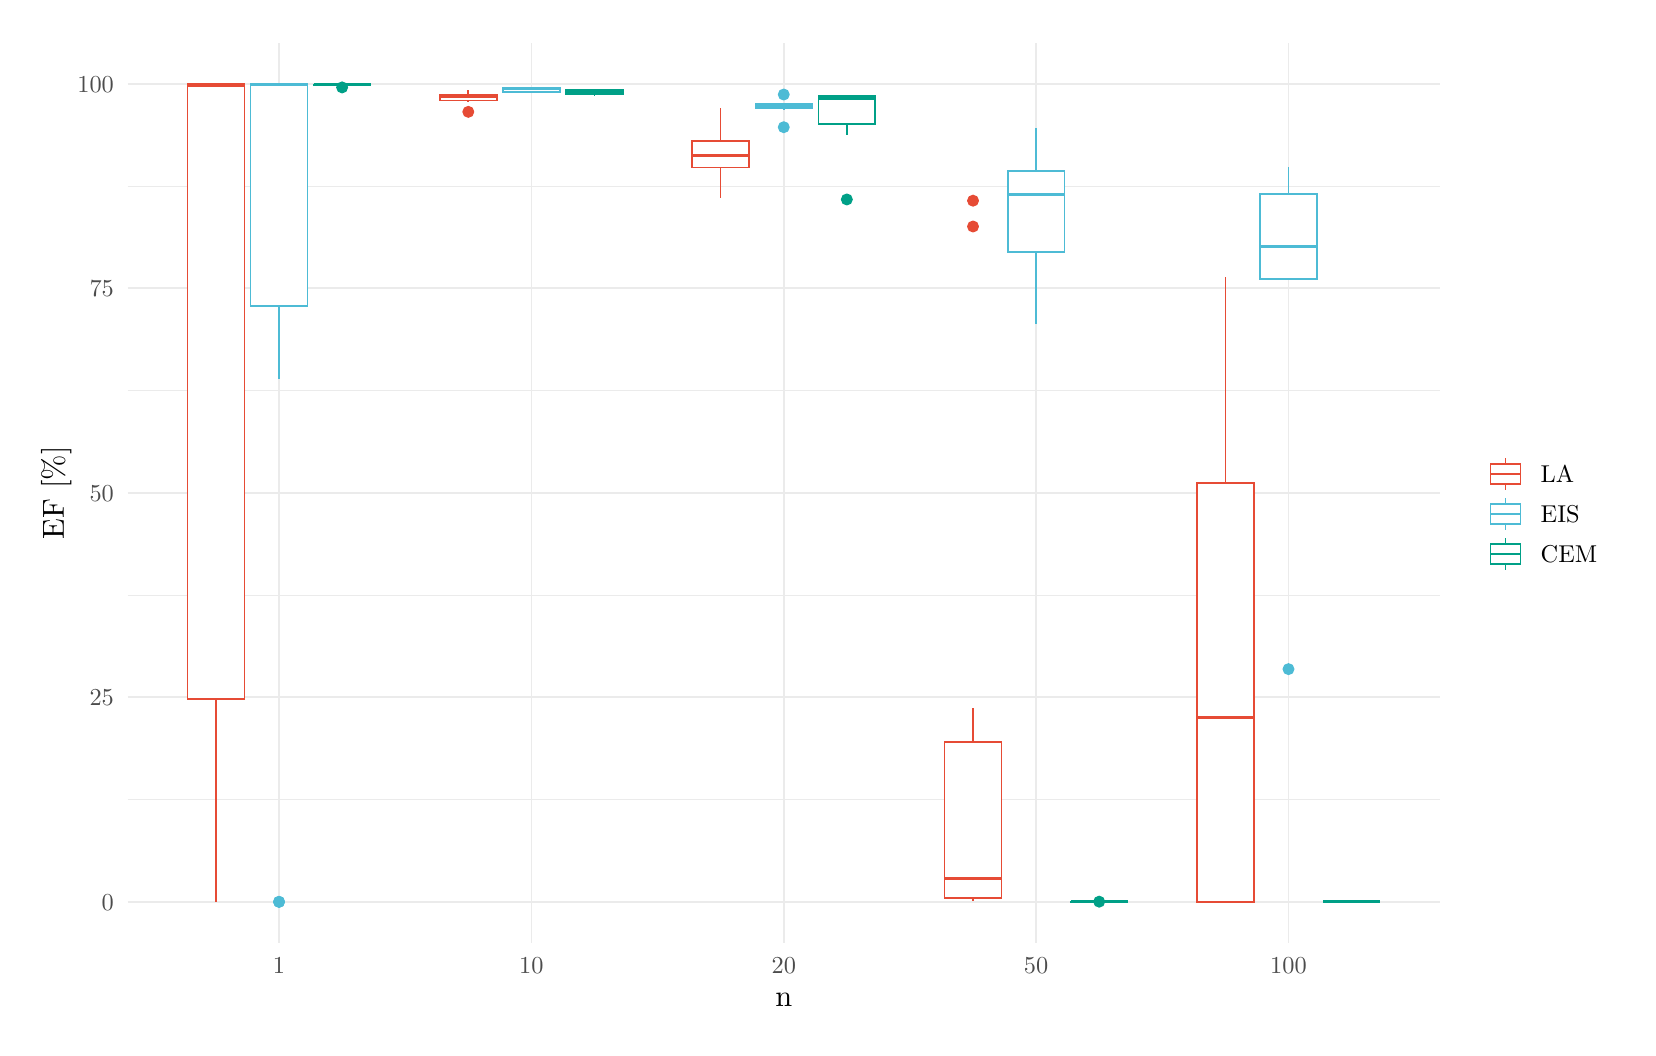
\begin{tikzpicture}[x=1pt,y=1pt]
\definecolor{fillColor}{RGB}{255,255,255}
\path[use as bounding box,fill=fillColor,fill opacity=0.00] (0,0) rectangle (578.16,361.35);
\begin{scope}
\path[clip] ( 36.11, 30.69) rectangle (510.30,355.85);
\definecolor{drawColor}{gray}{0.92}

\path[draw=drawColor,line width= 0.3pt,line join=round] ( 36.11, 82.42) --
	(510.30, 82.42);

\path[draw=drawColor,line width= 0.3pt,line join=round] ( 36.11,156.33) --
	(510.30,156.33);

\path[draw=drawColor,line width= 0.3pt,line join=round] ( 36.11,230.24) --
	(510.30,230.24);

\path[draw=drawColor,line width= 0.3pt,line join=round] ( 36.11,304.15) --
	(510.30,304.15);

\path[draw=drawColor,line width= 0.6pt,line join=round] ( 36.11, 45.46) --
	(510.30, 45.46);

\path[draw=drawColor,line width= 0.6pt,line join=round] ( 36.11,119.37) --
	(510.30,119.37);

\path[draw=drawColor,line width= 0.6pt,line join=round] ( 36.11,193.28) --
	(510.30,193.28);

\path[draw=drawColor,line width= 0.6pt,line join=round] ( 36.11,267.20) --
	(510.30,267.20);

\path[draw=drawColor,line width= 0.6pt,line join=round] ( 36.11,341.11) --
	(510.30,341.11);

\path[draw=drawColor,line width= 0.6pt,line join=round] ( 90.83, 30.69) --
	( 90.83,355.85);

\path[draw=drawColor,line width= 0.6pt,line join=round] (182.02, 30.69) --
	(182.02,355.85);

\path[draw=drawColor,line width= 0.6pt,line join=round] (273.21, 30.69) --
	(273.21,355.85);

\path[draw=drawColor,line width= 0.6pt,line join=round] (364.40, 30.69) --
	(364.40,355.85);

\path[draw=drawColor,line width= 0.6pt,line join=round] (455.59, 30.69) --
	(455.59,355.85);
\definecolor{drawColor}{RGB}{230,75,53}

\path[draw=drawColor,line width= 0.6pt,line join=round] ( 68.03,340.88) -- ( 68.03,341.02);

\path[draw=drawColor,line width= 0.6pt,line join=round] ( 68.03,118.83) -- ( 68.03, 45.47);
\definecolor{fillColor}{RGB}{255,255,255}

\path[draw=drawColor,line width= 0.6pt,fill=fillColor] ( 57.77,340.88) --
	( 57.77,118.83) --
	( 78.29,118.83) --
	( 78.29,340.88) --
	( 57.77,340.88) --
	cycle;

\path[draw=drawColor,line width= 1.1pt] ( 57.77,340.58) -- ( 78.29,340.58);
\definecolor{fillColor}{RGB}{230,75,53}

\path[draw=drawColor,line width= 0.4pt,line join=round,line cap=round,fill=fillColor] (159.22,330.93) circle (  1.96);

\path[draw=drawColor,line width= 0.6pt,line join=round] (159.22,337.23) -- (159.22,338.73);

\path[draw=drawColor,line width= 0.6pt,line join=round] (159.22,334.99) -- (159.22,334.73);
\definecolor{fillColor}{RGB}{255,255,255}

\path[draw=drawColor,line width= 0.6pt,fill=fillColor] (148.96,337.23) --
	(148.96,334.99) --
	(169.48,334.99) --
	(169.48,337.23) --
	(148.96,337.23) --
	cycle;

\path[draw=drawColor,line width= 1.1pt] (148.96,336.59) -- (169.48,336.59);

\path[draw=drawColor,line width= 0.6pt,line join=round] (250.41,320.30) -- (250.41,332.48);

\path[draw=drawColor,line width= 0.6pt,line join=round] (250.41,310.76) -- (250.41,299.67);

\path[draw=drawColor,line width= 0.6pt,fill=fillColor] (240.15,320.30) --
	(240.15,310.76) --
	(260.67,310.76) --
	(260.67,320.30) --
	(240.15,320.30) --
	cycle;

\path[draw=drawColor,line width= 1.1pt] (240.15,315.27) -- (260.67,315.27);
\definecolor{fillColor}{RGB}{230,75,53}

\path[draw=drawColor,line width= 0.4pt,line join=round,line cap=round,fill=fillColor] (341.60,289.50) circle (  1.96);

\path[draw=drawColor,line width= 0.4pt,line join=round,line cap=round,fill=fillColor] (341.60,298.83) circle (  1.96);

\path[draw=drawColor,line width= 0.6pt,line join=round] (341.60,103.29) -- (341.60,115.37);

\path[draw=drawColor,line width= 0.6pt,line join=round] (341.60, 46.75) -- (341.60, 45.65);
\definecolor{fillColor}{RGB}{255,255,255}

\path[draw=drawColor,line width= 0.6pt,fill=fillColor] (331.34,103.29) --
	(331.34, 46.75) --
	(351.86, 46.75) --
	(351.86,103.29) --
	(331.34,103.29) --
	cycle;

\path[draw=drawColor,line width= 1.1pt] (331.34, 53.99) -- (351.86, 53.99);

\path[draw=drawColor,line width= 0.6pt,line join=round] (432.79,196.92) -- (432.79,271.42);

\path[draw=drawColor,line width= 0.6pt,line join=round] (432.79, 45.49) -- (432.79, 45.47);

\path[draw=drawColor,line width= 0.6pt,fill=fillColor] (422.53,196.92) --
	(422.53, 45.49) --
	(443.05, 45.49) --
	(443.05,196.92) --
	(422.53,196.92) --
	cycle;

\path[draw=drawColor,line width= 1.1pt] (422.53,111.95) -- (443.05,111.95);
\definecolor{drawColor}{RGB}{77,187,213}
\definecolor{fillColor}{RGB}{77,187,213}

\path[draw=drawColor,line width= 0.4pt,line join=round,line cap=round,fill=fillColor] ( 90.83, 45.47) circle (  1.96);

\path[draw=drawColor,line width= 0.4pt,line join=round,line cap=round,fill=fillColor] ( 90.83, 45.47) circle (  1.96);

\path[draw=drawColor,line width= 0.6pt,line join=round] ( 90.83,341.00) -- ( 90.83,341.07);

\path[draw=drawColor,line width= 0.6pt,line join=round] ( 90.83,260.86) -- ( 90.83,234.38);
\definecolor{fillColor}{RGB}{255,255,255}

\path[draw=drawColor,line width= 0.6pt,fill=fillColor] ( 80.57,341.00) --
	( 80.57,260.86) --
	(101.08,260.86) --
	(101.08,341.00) --
	( 80.57,341.00) --
	cycle;

\path[draw=drawColor,line width= 1.1pt] ( 80.57,340.73) -- (101.08,340.73);

\path[draw=drawColor,line width= 0.6pt,line join=round] (182.02,339.44) -- (182.02,340.00);

\path[draw=drawColor,line width= 0.6pt,line join=round] (182.02,338.20) -- (182.02,337.65);

\path[draw=drawColor,line width= 0.6pt,fill=fillColor] (171.76,339.44) --
	(171.76,338.20) --
	(192.27,338.20) --
	(192.27,339.44) --
	(171.76,339.44) --
	cycle;

\path[draw=drawColor,line width= 1.1pt] (171.76,339.21) -- (192.27,339.21);
\definecolor{fillColor}{RGB}{77,187,213}

\path[draw=drawColor,line width= 0.4pt,line join=round,line cap=round,fill=fillColor] (273.21,325.38) circle (  1.96);

\path[draw=drawColor,line width= 0.4pt,line join=round,line cap=round,fill=fillColor] (273.21,337.19) circle (  1.96);

\path[draw=drawColor,line width= 0.6pt,line join=round] (273.21,333.78) -- (273.21,333.83);

\path[draw=drawColor,line width= 0.6pt,line join=round] (273.21,332.32) -- (273.21,331.55);
\definecolor{fillColor}{RGB}{255,255,255}

\path[draw=drawColor,line width= 0.6pt,fill=fillColor] (262.95,333.78) --
	(262.95,332.32) --
	(283.46,332.32) --
	(283.46,333.78) --
	(262.95,333.78) --
	cycle;

\path[draw=drawColor,line width= 1.1pt] (262.95,332.77) -- (283.46,332.77);

\path[draw=drawColor,line width= 0.6pt,line join=round] (364.40,309.53) -- (364.40,325.14);

\path[draw=drawColor,line width= 0.6pt,line join=round] (364.40,280.21) -- (364.40,254.37);

\path[draw=drawColor,line width= 0.6pt,fill=fillColor] (354.14,309.53) --
	(354.14,280.21) --
	(374.65,280.21) --
	(374.65,309.53) --
	(354.14,309.53) --
	cycle;

\path[draw=drawColor,line width= 1.1pt] (354.14,301.04) -- (374.65,301.04);
\definecolor{fillColor}{RGB}{77,187,213}

\path[draw=drawColor,line width= 0.4pt,line join=round,line cap=round,fill=fillColor] (455.59,129.56) circle (  1.96);

\path[draw=drawColor,line width= 0.6pt,line join=round] (455.59,301.18) -- (455.59,311.12);

\path[draw=drawColor,line width= 0.6pt,line join=round] (455.59,270.50) -- (455.59,270.13);
\definecolor{fillColor}{RGB}{255,255,255}

\path[draw=drawColor,line width= 0.6pt,fill=fillColor] (445.33,301.18) --
	(445.33,270.50) --
	(465.84,270.50) --
	(465.84,301.18) --
	(445.33,301.18) --
	cycle;

\path[draw=drawColor,line width= 1.1pt] (445.33,282.27) -- (465.84,282.27);
\definecolor{drawColor}{RGB}{0,160,135}
\definecolor{fillColor}{RGB}{0,160,135}

\path[draw=drawColor,line width= 0.4pt,line join=round,line cap=round,fill=fillColor] (113.62,339.76) circle (  1.96);

\path[draw=drawColor,line width= 0.6pt,line join=round] (113.62,340.86) -- (113.62,340.98);

\path[draw=drawColor,line width= 0.6pt,line join=round] (113.62,340.51) -- (113.62,340.26);
\definecolor{fillColor}{RGB}{255,255,255}

\path[draw=drawColor,line width= 0.6pt,fill=fillColor] (103.36,340.86) --
	(103.36,340.51) --
	(123.88,340.51) --
	(123.88,340.86) --
	(103.36,340.86) --
	cycle;

\path[draw=drawColor,line width= 1.1pt] (103.36,340.75) -- (123.88,340.75);

\path[draw=drawColor,line width= 0.6pt,line join=round] (204.81,338.77) -- (204.81,339.34);

\path[draw=drawColor,line width= 0.6pt,line join=round] (204.81,337.35) -- (204.81,336.71);

\path[draw=drawColor,line width= 0.6pt,fill=fillColor] (194.55,338.77) --
	(194.55,337.35) --
	(215.07,337.35) --
	(215.07,338.77) --
	(194.55,338.77) --
	cycle;

\path[draw=drawColor,line width= 1.1pt] (194.55,337.93) -- (215.07,337.93);
\definecolor{fillColor}{RGB}{0,160,135}

\path[draw=drawColor,line width= 0.4pt,line join=round,line cap=round,fill=fillColor] (296.00,299.27) circle (  1.96);

\path[draw=drawColor,line width= 0.6pt,line join=round] (296.00,336.58) -- (296.00,336.88);

\path[draw=drawColor,line width= 0.6pt,line join=round] (296.00,326.48) -- (296.00,322.44);
\definecolor{fillColor}{RGB}{255,255,255}

\path[draw=drawColor,line width= 0.6pt,fill=fillColor] (285.74,336.58) --
	(285.74,326.48) --
	(306.26,326.48) --
	(306.26,336.58) --
	(285.74,336.58) --
	cycle;

\path[draw=drawColor,line width= 1.1pt] (285.74,335.83) -- (306.26,335.83);
\definecolor{fillColor}{RGB}{0,160,135}

\path[draw=drawColor,line width= 0.4pt,line join=round,line cap=round,fill=fillColor] (387.19, 45.53) circle (  1.96);

\path[draw=drawColor,line width= 0.6pt,line join=round] (387.19, 45.49) -- (387.19, 45.49);

\path[draw=drawColor,line width= 0.6pt,line join=round] (387.19, 45.47) -- (387.19, 45.47);
\definecolor{fillColor}{RGB}{255,255,255}

\path[draw=drawColor,line width= 0.6pt,fill=fillColor] (376.93, 45.49) --
	(376.93, 45.47) --
	(397.45, 45.47) --
	(397.45, 45.49) --
	(376.93, 45.49) --
	cycle;

\path[draw=drawColor,line width= 1.1pt] (376.93, 45.49) -- (397.45, 45.49);

\path[draw=drawColor,line width= 0.6pt,line join=round] (478.38, 45.51) -- (478.38, 45.51);

\path[draw=drawColor,line width= 0.6pt,line join=round] (478.38, 45.51) -- (478.38, 45.51);

\path[draw=drawColor,line width= 0.6pt,fill=fillColor] (468.12, 45.51) --
	(468.12, 45.51) --
	(488.64, 45.51) --
	(488.64, 45.51) --
	(468.12, 45.51) --
	cycle;

\path[draw=drawColor,line width= 1.1pt] (468.12, 45.51) -- (488.64, 45.51);
\end{scope}
\begin{scope}
\path[clip] (  0.00,  0.00) rectangle (578.16,361.35);
\definecolor{drawColor}{gray}{0.30}

\node[text=drawColor,anchor=base east,inner sep=0pt, outer sep=0pt, scale=  0.88] at ( 31.16, 42.43) {0};

\node[text=drawColor,anchor=base east,inner sep=0pt, outer sep=0pt, scale=  0.88] at ( 31.16,116.34) {25};

\node[text=drawColor,anchor=base east,inner sep=0pt, outer sep=0pt, scale=  0.88] at ( 31.16,190.25) {50};

\node[text=drawColor,anchor=base east,inner sep=0pt, outer sep=0pt, scale=  0.88] at ( 31.16,264.17) {75};

\node[text=drawColor,anchor=base east,inner sep=0pt, outer sep=0pt, scale=  0.88] at ( 31.16,338.08) {100};
\end{scope}
\begin{scope}
\path[clip] (  0.00,  0.00) rectangle (578.16,361.35);
\definecolor{drawColor}{gray}{0.30}

\node[text=drawColor,anchor=base,inner sep=0pt, outer sep=0pt, scale=  0.88] at ( 90.83, 19.68) {1};

\node[text=drawColor,anchor=base,inner sep=0pt, outer sep=0pt, scale=  0.88] at (182.02, 19.68) {10};

\node[text=drawColor,anchor=base,inner sep=0pt, outer sep=0pt, scale=  0.88] at (273.21, 19.68) {20};

\node[text=drawColor,anchor=base,inner sep=0pt, outer sep=0pt, scale=  0.88] at (364.40, 19.68) {50};

\node[text=drawColor,anchor=base,inner sep=0pt, outer sep=0pt, scale=  0.88] at (455.59, 19.68) {100};
\end{scope}
\begin{scope}
\path[clip] (  0.00,  0.00) rectangle (578.16,361.35);
\definecolor{drawColor}{RGB}{0,0,0}

\node[text=drawColor,anchor=base,inner sep=0pt, outer sep=0pt, scale=  1.10] at (273.21,  7.64) {n};
\end{scope}
\begin{scope}
\path[clip] (  0.00,  0.00) rectangle (578.16,361.35);
\definecolor{drawColor}{RGB}{0,0,0}

\node[text=drawColor,rotate= 90.00,anchor=base,inner sep=0pt, outer sep=0pt, scale=  1.10] at ( 13.08,193.27) {EF [\%]};
\end{scope}
\begin{scope}
\path[clip] (  0.00,  0.00) rectangle (578.16,361.35);
\definecolor{drawColor}{RGB}{230,75,53}

\path[draw=drawColor,line width= 0.6pt] (534.03,194.33) --
	(534.03,196.50);

\path[draw=drawColor,line width= 0.6pt] (534.03,203.73) --
	(534.03,205.90);
\definecolor{fillColor}{RGB}{255,255,255}

\path[draw=drawColor,line width= 0.6pt,fill=fillColor] (528.61,196.50) rectangle (539.45,203.73);

\path[draw=drawColor,line width= 0.6pt] (528.61,200.11) --
	(539.45,200.11);
\end{scope}
\begin{scope}
\path[clip] (  0.00,  0.00) rectangle (578.16,361.35);
\definecolor{drawColor}{RGB}{77,187,213}

\path[draw=drawColor,line width= 0.6pt] (534.03,179.88) --
	(534.03,182.05);

\path[draw=drawColor,line width= 0.6pt] (534.03,189.27) --
	(534.03,191.44);
\definecolor{fillColor}{RGB}{255,255,255}

\path[draw=drawColor,line width= 0.6pt,fill=fillColor] (528.61,182.05) rectangle (539.45,189.27);

\path[draw=drawColor,line width= 0.6pt] (528.61,185.66) --
	(539.45,185.66);
\end{scope}
\begin{scope}
\path[clip] (  0.00,  0.00) rectangle (578.16,361.35);
\definecolor{drawColor}{RGB}{0,160,135}

\path[draw=drawColor,line width= 0.6pt] (534.03,165.43) --
	(534.03,167.59);

\path[draw=drawColor,line width= 0.6pt] (534.03,174.82) --
	(534.03,176.99);
\definecolor{fillColor}{RGB}{255,255,255}

\path[draw=drawColor,line width= 0.6pt,fill=fillColor] (528.61,167.59) rectangle (539.45,174.82);

\path[draw=drawColor,line width= 0.6pt] (528.61,171.21) --
	(539.45,171.21);
\end{scope}
\begin{scope}
\path[clip] (  0.00,  0.00) rectangle (578.16,361.35);
\definecolor{drawColor}{RGB}{0,0,0}

\node[text=drawColor,anchor=base west,inner sep=0pt, outer sep=0pt, scale=  0.88] at (546.75,197.08) {LA};
\end{scope}
\begin{scope}
\path[clip] (  0.00,  0.00) rectangle (578.16,361.35);
\definecolor{drawColor}{RGB}{0,0,0}

\node[text=drawColor,anchor=base west,inner sep=0pt, outer sep=0pt, scale=  0.88] at (546.75,182.63) {EIS};
\end{scope}
\begin{scope}
\path[clip] (  0.00,  0.00) rectangle (578.16,361.35);
\definecolor{drawColor}{RGB}{0,0,0}

\node[text=drawColor,anchor=base west,inner sep=0pt, outer sep=0pt, scale=  0.88] at (546.75,168.18) {CEM};
\end{scope}
\end{tikzpicture}
